\documentclass[
    language=english,
    doctype=comic-book,
    institution=none,
]{../../omnilatex}

\RequirePackage{config/document-settings}
\usepackage{tikz}
\usetikzlibrary{shapes, positioning, calc, decorations.pathmorphing, backgrounds}

\begin{document}
\maketitle

\vspace{1cm}

\begin{center}
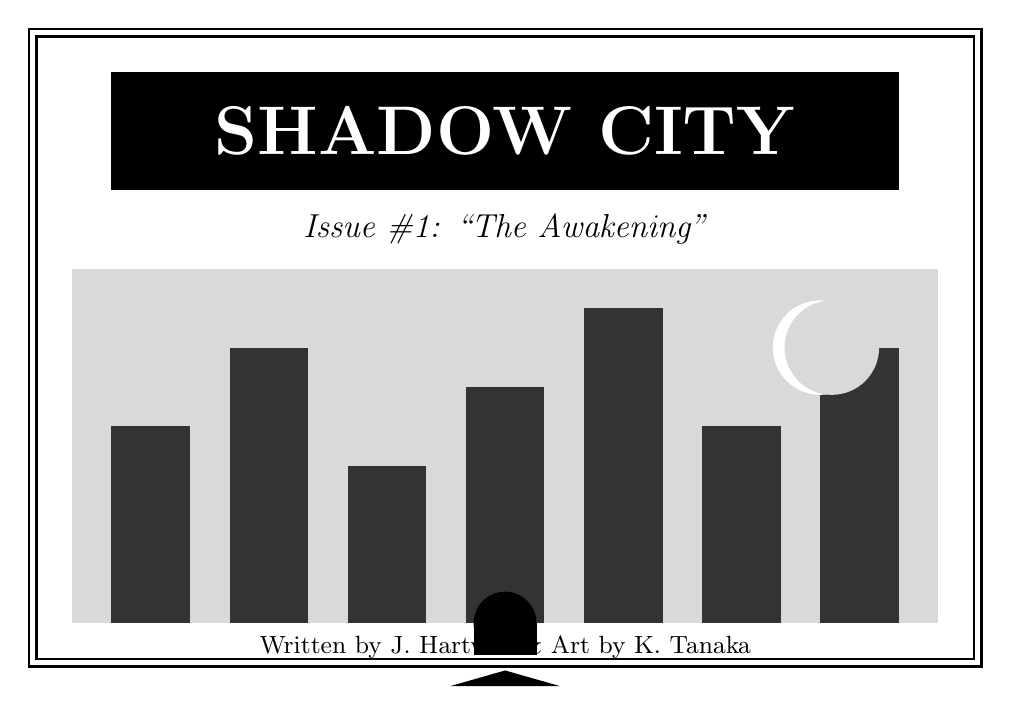
\begin{tikzpicture}
    % Cover illustration frame
    \draw[thick, double, double distance=2pt] (0,0) rectangle (12,8);
    
    % Title banner
    \fill[black] (1,6) rectangle (11,7.5);
    \node[white, font=\Huge\bfseries] at (6,6.75) {SHADOW CITY};
    
    % Subtitle
    \node[font=\large\itshape] at (6,5.5) {Issue \#1: ``The Awakening''};
    
    % Cover image placeholder - cityscape
    \fill[gray!30] (0.5,0.5) rectangle (11.5,5);
    
    % Simple cityscape silhouette
    \fill[black!80] (1,0.5) rectangle (2,3);
    \fill[black!80] (2.5,0.5) rectangle (3.5,4);
    \fill[black!80] (4,0.5) rectangle (5,2.5);
    \fill[black!80] (5.5,0.5) rectangle (6.5,3.5);
    \fill[black!80] (7,0.5) rectangle (8,4.5);
    \fill[black!80] (8.5,0.5) rectangle (9.5,3);
    \fill[black!80] (10,0.5) rectangle (11,4);
    
    % Moon
    \fill[white] (10,4) circle (0.6);
    \fill[gray!30] (10.15,4) circle (0.6);
    
    % Figure silhouette
    \fill[black] (6,0.5) circle (0.4); % head
    \fill[black] (5.6,0.1) rectangle (6.4,0.5); % body
    \fill[black] (5.3,-0.3) -- (6,-0.1) -- (6.7,-0.3) -- cycle; % cape
    
    % Credit
    \node[font=\small] at (6,0.2) {Written by J. Hartwell \& Art by K. Tanaka};
\end{tikzpicture}
\end{center}

\vspace{1cm}

\section*{CHARACTERS}

\begin{itemize}
    \item \textbf{KAI NOVA} (25) --- A street artist with the ability to bring her drawings to life. Wears a black hoodie and carries a bag of markers.
    \item \textbf{THE COLLECTOR} (ageless) --- A shadowy figure who absorbs memories through physical touch. Drains color from everything he touches.
    \item \textbf{DETECTIVE SARAH CHEN} (40s) --- A skeptical police detective investigating the string of ``color theft'' incidents.
    \item \textbf{MR. INKWELL} (70s) --- A mysterious art supplies shop owner who knows more than he lets on.
\end{itemize}

\chapter{PAGE ONE}

\begin{center}
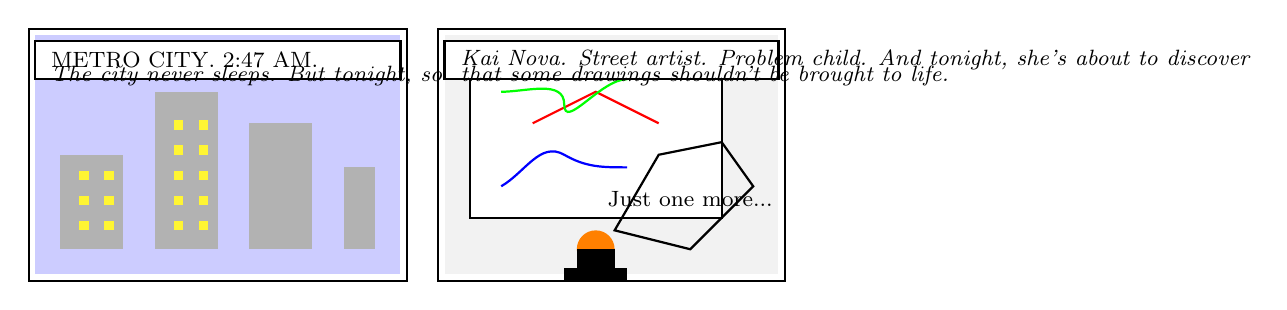
\begin{tikzpicture}[scale=0.8]
    % Panel 1 - establishing shot
    \draw[thick] (0,0) rectangle (6,4);
    \fill[blue!20] (0.1,0.1) rectangle (5.9,3.9);
    
    % City buildings
    \fill[gray!60] (0.5,0.5) rectangle (1.5,2);
    \fill[gray!60] (2,0.5) rectangle (3,3);
    \fill[gray!60] (3.5,0.5) rectangle (4.5,2.5);
    \fill[gray!60] (5,0.5) rectangle (5.5,1.8);
    
    % Windows (yellow dots)
    \foreach \x in {0.8,1.2} {
        \foreach \y in {0.8,1.2,1.6} {
            \fill[yellow!80] (\x,\y) rectangle (\x+0.15,\y+0.15);
        }
    }
    \foreach \x in {2.3,2.7} {
        \foreach \y in {0.8,1.2,1.6,2.0,2.4} {
            \fill[yellow!80] (\x,\y) rectangle (\x+0.15,\y+0.15);
        }
    }
    
    % Narration box
    \fill[white, draw=black, thick] (0.1,3.2) rectangle (5.9,3.8);
    \node[anchor=west, font=\footnotesize] at (0.2,3.5) {METRO CITY. 2:47 AM.};
    \node[anchor=west, font=\footnotesize\itshape] at (0.2,3.25) {The city never sleeps. But tonight, something is waking up.};
    
    % Panel 2 - Kai drawing
    \draw[thick] (6.5,0) rectangle (12,4);
    \fill[gray!10] (6.6,0.1) rectangle (11.9,3.9);
    
    % Kai figure
    \fill[orange] (9,0.5) circle (0.3); % head
    \fill[black] (8.7,0.2) rectangle (9.3,0.5); % body
    \fill[black] (8.5,0) rectangle (9.5,0.2); % legs
    
    % Drawing on wall
    \fill[white] (7,1) rectangle (11,3.5);
    \draw[thick] (7,1) rectangle (11,3.5);
    
    % Scribbles on wall
    \draw[thick, blue] (7.5,1.5) to[out=30,in=150] (8.5,2) to[out=-30,in=180] (9.5,1.8);
    \draw[thick, red] (8,2.5) -- (9,3) -- (10,2.5);
    \draw[thick, green] (7.5,3) to[out=0,in=90] (8.5,2.8) to[out=-90,in=180] (9.5,3.2);
    
    % Speech bubble
    \draw[thick] (9.3,0.8) -- (10,2) -- (11,2.2) -- (11.5,1.5) -- (10.5,0.5) -- cycle;
    \node[anchor=center, font=\footnotesize] at (10.5,1.3) {Just one more...};
    
    % Narration
    \fill[white, draw=black, thick] (6.6,3.2) rectangle (11.9,3.8);
    \node[anchor=west, font=\footnotesize\itshape] at (6.7,3.5) {Kai Nova. Street artist. Problem child. And tonight, she's about to discover};
    \node[anchor=west, font=\footnotesize\itshape] at (6.7,3.25) {that some drawings shouldn't be brought to life.};
\end{tikzpicture}
\end{center}

\vspace{0.5cm}

\begin{quote}
\textbf{KAI (V.O.):} They say the city is a canvas. That every wall is a page waiting to be written on. They're wrong. The city isn't a canvas. It's a prison. And the walls aren't waiting to be written on---they're waiting to be broken.
\end{quote}

\begin{quote}
\textbf{KAI (V.O.):} My name is Kai Nova. I draw things. And sometimes---when the markers are right, when the wall is ready, when the moon is in the right part of the sky---the things I draw... wake up.
\end{quote}

\chapter{PAGE TWO}

\begin{center}
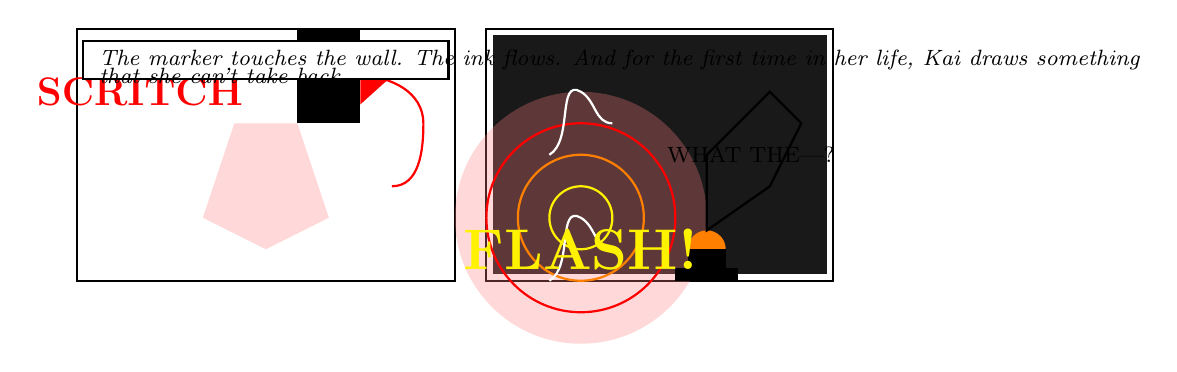
\begin{tikzpicture}[scale=0.8]
    % Panel 1 - close up of marker touching wall
    \draw[thick] (0,0) rectangle (6,4);
    \fill[white] (0.1,0.1) rectangle (5.9,3.9);
    
    % Hand with marker
    \fill[pink!60] (2,1) -- (3,0.5) -- (4,1) -- (3.5,2.5) -- (2.5,2.5) -- cycle;
    
    % Marker
    \fill[black] (3.5,2.5) rectangle (4.5,4);
    \fill[red] (4.5,2.8) -- (5,3.25) -- (4.5,3.7);
    
    % Ink trail
    \draw[thick, red] (4.5,3.25) to[out=0,in=90] (5.5,2.5) to[out=-90,in=0] (5,1.5);
    
    % Sound effect
    \node[font=\Large\bfseries, red] at (1,3) {SCRITCH};
    
    % Panel 2 - the drawing comes alive
    \draw[thick] (6.5,0) rectangle (12,4);
    \fill[black!90] (6.6,0.1) rectangle (11.9,3.9);
    
    % Glowing drawing
    \fill[red!50, opacity=0.3] (8,1) circle (2);
    \draw[thick, red, thick] (8,1) circle (1.5);
    \draw[thick, orange] (8,1) circle (1);
    \draw[thick, yellow] (8,1) circle (0.5);
    
    % Drawing figure emerging
    \draw[thick, white] (7.5,2) to[out=30,in=150] (8,3) to[out=-30,in=180] (8.5,2.5);
    \draw[thick, white] (7.5,0) to[out=30,in=150] (8,1) to[out=-30,in=180] (8.5,0.5);
    
    % Kai's reaction
    \fill[orange] (10,0.5) circle (0.3);
    \fill[black] (9.7,0.2) rectangle (10.3,0.5);
    \fill[black] (9.5,0) rectangle (10.5,0.2);
    
    % Speech bubble
    \draw[thick] (10,0.8) -- (11,1.5) -- (11.5,2.5) -- (11,3) -- (10,2) -- cycle;
    \node[anchor=center, font=\footnotesize] at (10.7,2) {WHAT THE---?};
    
    % Sound effect
    \node[font=\huge\bfseries, yellow] at (8,0.5) {FLASH!};
    
    % Narration
    \fill[white, draw=black, thick] (0.1,3.2) rectangle (5.9,3.8);
    \node[anchor=west, font=\footnotesize\itshape] at (0.2,3.5) {The marker touches the wall. The ink flows. And for the first time in her life, Kai draws something};
    \node[anchor=west, font=\footnotesize\itshape] at (0.2,3.25) {that she can't take back.};
\end{tikzpicture}
\end{center}

\vspace{0.5cm}

\begin{quote}
\textbf{KAI (V.O.):} I've been drawing since I was five. Chalk on sidewalks. Markers on walls. Paint on canvas. I've filled every surface in this city with something---tags, murals, portraits,抽象. But I've never drawn anything that looked back at me.
\end{quote}

\begin{quote}
\textbf{KAI (V.O.):} Until tonight.
\end{quote}

\begin{quote}
\textbf{KAI:} Okay. Okay. Don't panic. This is not happening. This is NOT HAPPENING.
\end{quote}

\begin{quote}
\textbf{KAI:} (to the drawing) You're not real. You can't be real. I drew you with a---with a cheap marker from the dollar store. You don't just---you can't just---
\end{quote}

\begin{quote}
\textbf{THE DRAWING:} (tilting its head, curious) ...Can't what?
\end{quote}

\chapter{PAGE THREE}

\begin{center}
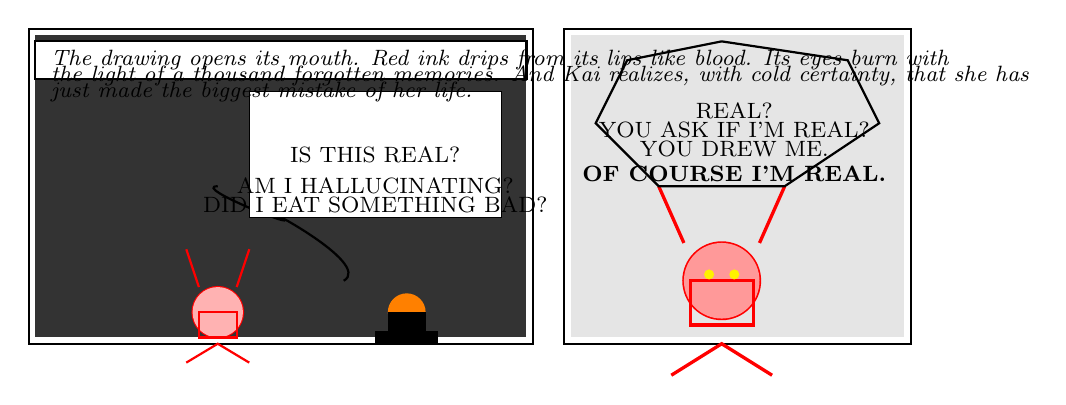
\begin{tikzpicture}[scale=0.8]
    % Panel 1 - Kai and the drawing face to face
    \draw[thick] (0,0) rectangle (8,5);
    \fill[black!80] (0.1,0.1) rectangle (7.9,4.9);
    
    % Drawing figure (more defined)
    \draw[thick, red] (3,0.5) circle (0.4);
    \fill[red!30] (3,0.5) circle (0.4);
    \draw[thick, red] (2.7,0.1) rectangle (3.3,0.5);
    \draw[thick, red] (2.5,-0.3) -- (3,0) -- (3.5,-0.3);
    \draw[thick, red] (2.7,0.9) -- (2.5,1.5);
    \draw[thick, red] (3.3,0.9) -- (3.5,1.5);
    
    % Kai (frozen in shock)
    \fill[orange] (6,0.5) circle (0.3);
    \fill[black] (5.7,0.2) rectangle (6.3,0.5);
    \fill[black] (5.5,0) rectangle (6.5,0.2);
    
    % Thought bubble
    \draw[thick] (5,1) to[out=30,in=150] (4,2) to[out=-30,in=180] (3,2.5);
    \fill[white, draw=black] (3.5,2) rectangle (7.5,4);
    \node[anchor=center, font=\footnotesize] at (5.5,3) {IS THIS REAL?};
    \node[anchor=center, font=\footnotesize] at (5.5,2.5) {AM I HALLUCINATING?};
    \node[anchor=center, font=\footnotesize] at (5.5,2.2) {DID I EAT SOMETHING BAD?};
    
    % Panel 2 - the drawing speaks
    \draw[thick] (8.5,0) rectangle (14,5);
    \fill[gray!20] (8.6,0.1) rectangle (13.9,4.9);
    
    % Drawing figure (larger, more menacing)
    \draw[thick, red, very thick] (11,1) circle (0.6);
    \fill[red!40] (11,1) circle (0.6);
    \draw[thick, red, very thick] (10.5,0.3) rectangle (11.5,1);
    \draw[thick, red, very thick] (10.2,-0.5) -- (11,0) -- (11.8,-0.5);
    \draw[thick, red, very thick] (10.4,1.6) -- (10,2.5);
    \draw[thick, red, very thick] (11.6,1.6) -- (12,2.5);
    
    % Eyes glowing
    \fill[yellow] (10.8,1.1) circle (0.08);
    \fill[yellow] (11.2,1.1) circle (0.08);
    
    % Speech bubble (jagged)
    \draw[thick] (10,2.5) -- (9,3.5) -- (9.5,4.5) -- (11,4.8) -- (13,4.5) -- (13.5,3.5) -- (12,2.5) -- cycle;
    \node[anchor=center, font=\footnotesize] at (11.2,3.7) {REAL?};
    \node[anchor=center, font=\footnotesize] at (11.2,3.4) {YOU ASK IF I'M REAL?};
    \node[anchor=center, font=\footnotesize] at (11.2,3.1) {YOU DREW ME.};
    \node[anchor=center, font=\footnotesize\bfseries] at (11.2,2.7) {OF COURSE I'M REAL.};
    
    % Narration
    \fill[white, draw=black, thick] (0.1,4.2) rectangle (7.9,4.8);
    \node[anchor=west, font=\footnotesize\itshape] at (0.2,4.5) {The drawing opens its mouth. Red ink drips from its lips like blood. Its eyes burn with};
    \node[anchor=west, font=\footnotesize\itshape] at (0.2,4.25) {the light of a thousand forgotten memories. And Kai realizes, with cold certainty, that she has};
    \node[anchor=west, font=\footnotesize\itshape] at (0.2,4.0) {just made the biggest mistake of her life.};
\end{tikzpicture}
\end{center}

\vspace{0.5cm}

\begin{quote}
\textbf{THE DRAWING:} My name is... I don't have a name. You didn't give me one. How rude. I think I'll choose my own.
\end{quote}

\begin{quote}
\textbf{THE DRAWING:} (looking at its hands) I am red. I am sharp. I am... angry. I think I'll call myself RED.
\end{quote}

\begin{quote}
\textbf{KAI:} Look, I don't know how you're doing this, but you need to go back. Back into the wall. Back into the ink. I didn't mean to---I was just practicing. I was just---
\end{quote}

\begin{quote}
\textbf{RED:} (stepping closer) Just what? Just playing? Just passing the time? You brought me into this world, Kai Nova. You gave me form. You gave me life. And now you want to send me back?
\end{quote}

\begin{quote}
\textbf{RED:} (leaning in, voice dropping) I don't think so.
\end{quote}

\begin{quote}
\textbf{KAI:} (backing away) How do you know my name?
\end{quote}

\begin{quote}
\textbf{RED:} (smiling, red ink dripping from its teeth) You drew me on the wall of your apartment building. The one with your name on the buzzer. I've been watching you for weeks, Kai. Waiting for you to bring me to life.
\end{quote}

\begin{quote}
\textbf{RED:} And now that I'm alive... I'm hungry.
\end{quote}

\begin{center}
\textbf{TO BE CONTINUED...}
\end{center}

\vspace{1cm}

\begin{center}
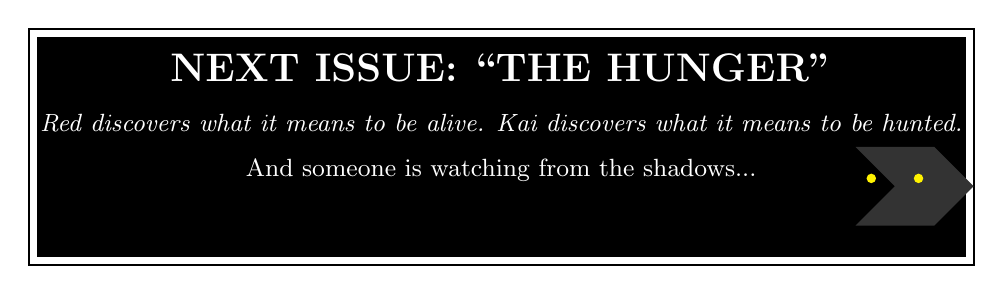
\begin{tikzpicture}
    % Next issue teaser
    \draw[thick] (0,0) rectangle (12,3);
    \fill[black] (0.1,0.1) rectangle (11.9,2.9);
    
    \node[white, font=\Large\bfseries] at (6,2.5) {NEXT ISSUE: ``THE HUNGER''};
    \node[white, font=\small\itshape] at (6,1.8) {Red discovers what it means to be alive. Kai discovers what it means to be hunted.};
    \node[white, font=\small] at (6,1.2) {And someone is watching from the shadows...};
    
    % Silhouette in corner
    \fill[black!80] (10.5,0.5) -- (11,1) -- (10.5,1.5) -- (11.5,1.5) -- (12,1) -- (11.5,0.5) -- cycle;
    \fill[yellow] (10.7,1.1) circle (0.06);
    \fill[yellow] (11.3,1.1) circle (0.06);
\end{tikzpicture}
\end{center}

\end{document}
